\documentclass{beamer}
\usepackage{multirow}
\usepackage{booktabs}
\usepackage[backend=biber,
style=authoryear-comp]{biblatex}

\usetheme{Madrid}

\bibliography{sample.bib} % Specify the bibliography file

\title{Systemic Risk and Financial Connectedness: Empirical Evidence}
\author{Mateusz Dadej}
\institute{Phd. student at Universita degli Studi di Brescia, ITA \\
Visiting researcher at Universität Mannheim, DE}

\setbeamertemplate{bibliography item}{}

\begin{document}

\titlepage

\begin{frame}{Theoretical background}   
    \begin{itemize}
        \item "robust-yet-fragile" property of financial system can serve at the same time as shock-absorbers and shock-amplifiers to the financial sector (\cite{haldane}).
        \item This makes the system robust, when the magnitude of shock is relatively small, but fragile, when the shock is large. 
        \item A seminal paper by \cite{acemoglu}, provides a formal model, in which an extent of financial contagion exhibits a form of regime transition.
            \begin{itemize}
                \item When the shocks are small, the damages are dissipated through large number of financial institutions.
                \item When the shock is above some threshold, the properties of the system changes markedly. The damages are amplified through the network.
            \end{itemize}
    
    \end{itemize}
\end{frame}

\begin{frame}{Research design}

    \begin{itemize}
        \item aim is to provide empirical evidence for the regime-dependent effect of connectedness on financial stability, i.e.:
        \begin{itemize}
            \item Stable markets regime: Higher connectedness -> less volatility
            \item High shock regime: Higher connectedness -> more volatility
        \end{itemize}
        \item In a following steps:
        \begin{itemize}
            \item Based on stock prices of the biggest banks in EU and USA, I calculate the connectedness (e.g. correlation) measure in a rolling window basis.
            \item This time series measure is then used as an explanatory variable in a Markov switching ARCH model.    
        \end{itemize}
    \end{itemize}
    
\end{frame}  

\begin{frame}{Connectedness measures - denoted $\kappa_t$}

    \begin{itemize}
        \item Average correlation: $\frac{\sum_{i \neq i}^{N} \sum_{j \neq j}^{N} \rho_{i,j}(R)}{N^2-N}$,  with $\rho(\cdot)$ being the Ledoit-Wolf estimator of the covariance matrix (\cite{ledoit}).
        \item $\frac{\sum_{i}^{k} \lambda_i}{\sum_{i}^{N} \lambda_i}$, with $\lambda$ being an eigenvalue of the covariance matrix. 
        \item (\cite{granger}) - based measure of connectedness:
        \begin{itemize}
            \item For each of stock pair estimate: $r_{i,t+1} = \beta_0 + \beta_1 r_{m, t} + \beta_2 r_{j, t}$
            \item The "causality" matrix is set as: $G_{i,j} = \begin{cases}
                1  & \text{if } \beta_2 \text{ is significant} \\
                0 & \text{otherwise}
              \end{cases} \forall i \neq j$
            \item As with before we calculate average connectedness: $\frac{\sum_{i \neq j}^{N} \sum_{j \neq i}^{N} G_{i,j}}{ N \times (N-1)}$
        \end{itemize}
    
        Last two measures are as described in \cite{billio}
    \end{itemize}

\end{frame}

\begin{frame}{Connectedness measures results}

    \begin{figure}[H]
        \caption{Standardized time series of connectedness measures for a rolling window of 63 trading days (quarter)}
        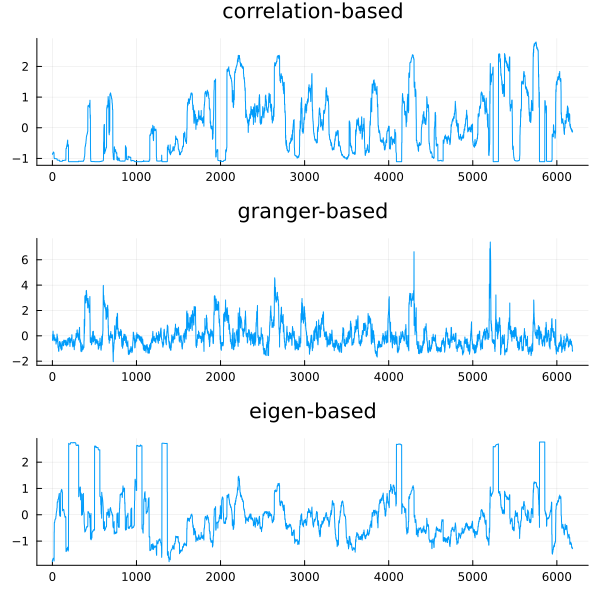
\includegraphics[scale=0.3]{connectmeasures.png}
        \centering
    \end{figure}    
\end{frame}    


\begin{frame}{Modeling the regime-dependent effect of connectedness}

    Mean specification of the model: 
    
    $$r_{b,t} = \beta_0 + \underbrace{\beta_1 r_{b,t-1}}_{\text{Banking index}} + \underbrace{\beta_2 r_{m,t-1}}_{\text{Broad market index}} + \epsilon_t$$
    
    The Markov-switching ARCH specification is:
    
    $$\sqrt{\epsilon^2_t} = \alpha_{0,s} + \underbrace{\alpha_{1,s}\kappa_{t-1}}_{\text{connectedness}} + \underbrace{\sum_{i=1}^{p} \alpha_{i+1} \sqrt{\epsilon^2_{t-i}}}_{\text{Lag controls}}$$
    
    
    With regime changes according to Markov process: \begin{equation*}
        P(S_t = i | S_{t-1} = j) = \begin{bmatrix}
          \pi_1 & 1 - \pi_2\\
            1 - \pi_1 & \pi_2
            \end{bmatrix}
    \end{equation*}
    
\end{frame}

\begin{frame}{Estimation results}
    EU banking sector and 252 trading days (year) rolling window 
    \begin{table}\small
        \begin{tabular}{cccccc}
          \toprule
           Connectedness measure &  & \multicolumn{2}{c}{\bfseries Regime 1} & \multicolumn{2}{c}{\bfseries Regime 2}  \\
           %\cmidrule(lr){1-6}
           \hline
           & & Estimate & S.E. & Estimate & S.E. \\
           \hline
           \multirow{3}{*}[\normalbaselineskip]{Correlation-based} & $\alpha_0$ & 0.466* & 0.019 & 1.988*  & 0.06 \\
            & $\alpha_1$ & 0.017 & 0.009 & 0.22* & 0.043 \\
            & $\eta$ & 0.435 & 0.009 & 1.4 & 0.012 \\
            & $\pi_{i,i}$ &  \multicolumn{2}{c}{78.6\%} & \multicolumn{2}{c}{52\%}\\
            \hline
            \multirow{3}{*}[\normalbaselineskip]{Eigenvalue-based} & $\alpha_0$ & 0.458* & 0.018 & 1.975*  & 0.061 \\
            & $\alpha_1$ & -0.002 & 0.008 & 0.052 & 0.048 \\
            & $\eta$ & 0.435 & 0.009 & 1.42 & 0.012 \\
            & $\pi_{i,i}$ &  \multicolumn{2}{c}{90\%} & \multicolumn{2}{c}{67.2\%}\\
            \hline
            \multirow{3}{*}[\normalbaselineskip]{Granger-based} & $\alpha_0$ & 0.468* & 0.018 & 1.984*  & 0.059 \\
            & $\alpha_1$ & 0.018* & 0.008 & 0.276* & 0.05 \\
            & $\eta$ & 0.433 & 0.009 & 1.394 & 0.013 \\
            & $\pi_{i,i}$ &  \multicolumn{2}{c}{78.5\%} & \multicolumn{2}{c}{52.5\%}\\
            \hline
          \multicolumn{6}{l}{\footnotesize * coefficient with 5\% statistical significance} \\
          \hline
        \end{tabular}
      \end{table}
\end{frame}  

\begin{frame}
    US banking sector and 63 trading days (year) rolling window
    \begin{table}\small
        \begin{tabular}{cccccc}
          \toprule
           Connectedness measure &  & \multicolumn{2}{c}{\bfseries Regime 1} & \multicolumn{2}{c}{\bfseries Regime 2}  \\
           %\cmidrule(lr){1-6}
           \hline
           & & Estimate & S.E. & Estimate & S.E. \\
           \hline
           \multirow{3}{*}[\normalbaselineskip]{Correlation-based} & $\alpha_0$ & 0.402* & 0.013 & 1.517*  & 0.054 \\
            & $\alpha_1$ & 0.027* & 0.007 & 0.239* & 0.044 \\
            & $\eta$ & 0.373 & 0.007 & 1.268 & 0.017 \\
            & $\pi_{i,i}$ &  \multicolumn{2}{c}{89.4\%} & \multicolumn{2}{c}{67\%}\\
            \hline
            \multirow{3}{*}[\normalbaselineskip]{Eigenvalue-based} & $\alpha_0$ & 0.416* & 0.014 & 1.554*  & 0.057 \\
            & $\alpha_1$ & 0.041* & 0.007 & 0.194* & 0.046 \\
            & $\eta$ & 0.38 & 0.006 & 1.304 & 0.016 \\
            & $\pi_{i,i}$ &  \multicolumn{2}{c}{90\%} & \multicolumn{2}{c}{67.2\%}\\
            \hline
            \multirow{3}{*}[\normalbaselineskip]{Granger-based} & $\alpha_0$ & 0.379* & 0.013 & 1.472*  & 0.047 \\
            & $\alpha_1$ & 0.009 & 0.007 & 0.205* & 0.032 \\
            & $\eta$ & 0.356 & 0.006 & 1.161 & 0.013 \\
            & $\pi_{i,i}$ &  \multicolumn{2}{c}{87.4\%} & \multicolumn{2}{c}{65\%}\\
            \hline
          \multicolumn{6}{l}{\footnotesize * coefficient with 5\% statistical significance} \\
          \hline
        \end{tabular}
      \end{table}

\end{frame}    

\begin{frame}[allowframebreaks]
    \frametitle{References}
      \printbibliography
\end{frame}


\end{document}